\documentclass{article}
\usepackage[utf8]{inputenc}
\usepackage{graphicx}
\usepackage{hyperref}

\title{CSI 5137 Ethics in AI Design Assignment 1}
\author{Massoud, Yahya 300147944 \and Zhang, Lingfeng 300134245 \and Zhou, Yiqiang 300129168}
\date{March 2020}

\begin{document}

\maketitle

\section{Final Value Map}

Our final value map with stakeholders, values and value tensions is in the google slides. The clickable link is \href{https://docs.google.com/presentation/d/1nQmXIbWmeZUNLPVEX4FJi_B35GRE-oLK9sPH9UOmlD0/edit?usp=sharing}{\url{https://docs.google.com/presentation/d/1nQmXIbWmeZUNLPVEX4FJi_B35GRE-oLK9sPH9UOmlD0/edit?usp=sharing}}. You can zoom in and out freely.

The illustrations of values and value tensions are all in slides.

\section{Stakeholders and values}

\begin{itemize}

\item owner of the house
\begin{itemize}
\item privacy
\item safety
\item convenience
\item entertainment
\item money saving
\item freedom of choice
\end{itemize}

\item Amazon company
\begin{itemize}
    \item responsibility
    \item trustworthiness
    \item creativity
    \item scalability
    \item leadership
    \item money
    \item restraint
    \item fidelity
    \item change
\end{itemize}

\item Amazon Echo Smart Speaker
\begin{itemize}
    \item usefulness
    \item self-control
\end{itemize}

\item family members: parents
\begin{itemize}
    \item protecting their kids(protection)
    \item control children's usage
    \item security of the home
    \item responsibility
    \item personal privacy
    \item convenience
    \item trustworthiness
    \item security
\end{itemize}

\item family members: children
\begin{itemize}
    \item freedom of using Alexa
    \item personal privacy
    \item companion
    \item safety
    \item entertainment
\end{itemize}

\item friends of the family
\begin{itemize}
    \item enjoyment
    \item sense of belonging
\end{itemize}

\item guests of the home
\begin{itemize}
    \item privacy
    \item convenience
\end{itemize}

\item advertisement companies
\begin{itemize}
    \item money
    \item accessibility
    \item data collection
    \item influence
\end{itemize}

\item smart devices(IoT)
\begin{itemize}
    \item usefulness
    \item self-control
\end{itemize}

\item software developer of Amazon echo smart speaker
\begin{itemize}
    \item skills
    \item data collection
    \item robustness
    \item data security
\end{itemize}

\item AI developer of Amazon echo smart speaker
\begin{itemize}
    \item accuracy
    \item precision
    \item generalization
    \item robustness
\end{itemize}

\item governments
\begin{itemize}
    \item duty
    \item regulation
    \item control
\end{itemize}

\item other traditional business companies, traditional companies who want to combine with AI
\begin{itemize}
    \item competition
    \item leadership
    \item growth
    \item money
    \item stability
    \item success
\end{itemize}

\item other traditional business companies,traditional companies who do not want to combine with AI

\item AWS

\item housekeeper

\item software developers of other companies who have developed Alexa
\begin{itemize}
    \item skills
    \item control
    \item freedom
    \item cooperation
    \item money
    \item profit
\end{itemize}

\item manufactories of other devices
\begin{itemize}
    \item focus
    \item flexibility
    \item cooperation
    \item variety
    \item independence
    \item innovation
    \item individuality
\end{itemize}

\item offline retailing stores
\begin{itemize}
    \item profits
    \item stability
    \item connection
    \item warm-heartness
    \item dominance
\end{itemize}
\end{itemize}

\section{Evidence of Design Iteration}

There are many iterations we have done.

Initially, we analysis the Amazon Echo ethics case, and wrote down stakeholders, values, value tensions. Draft graphs are shown below.

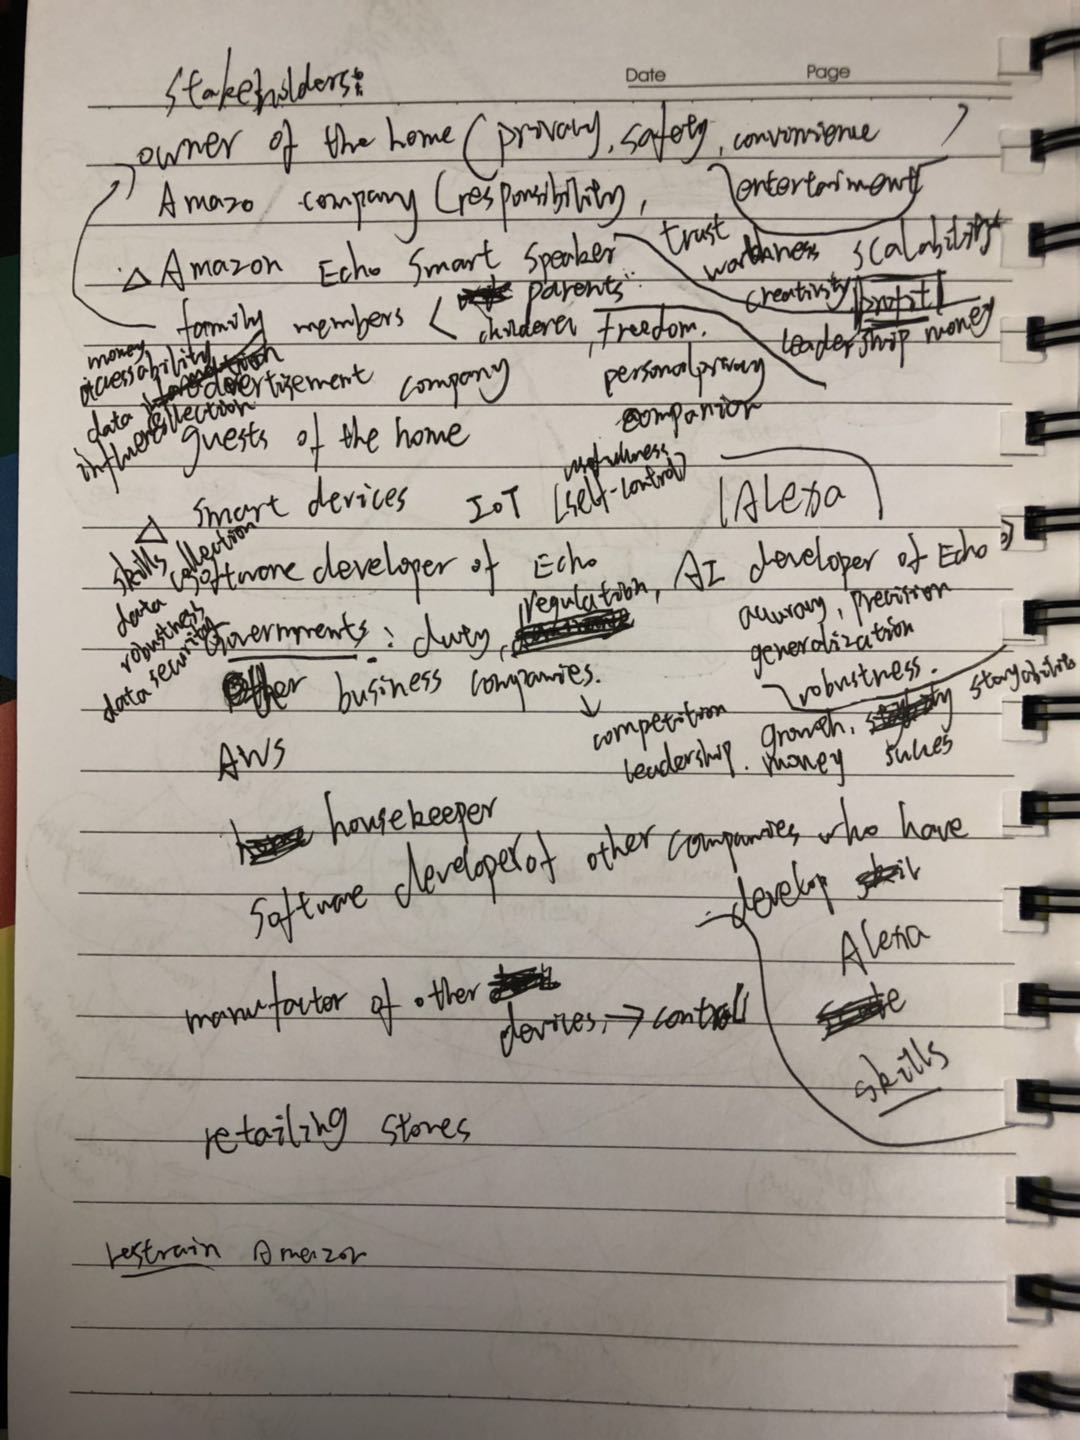
\includegraphics[scale=0.3]{values_1.jpeg}

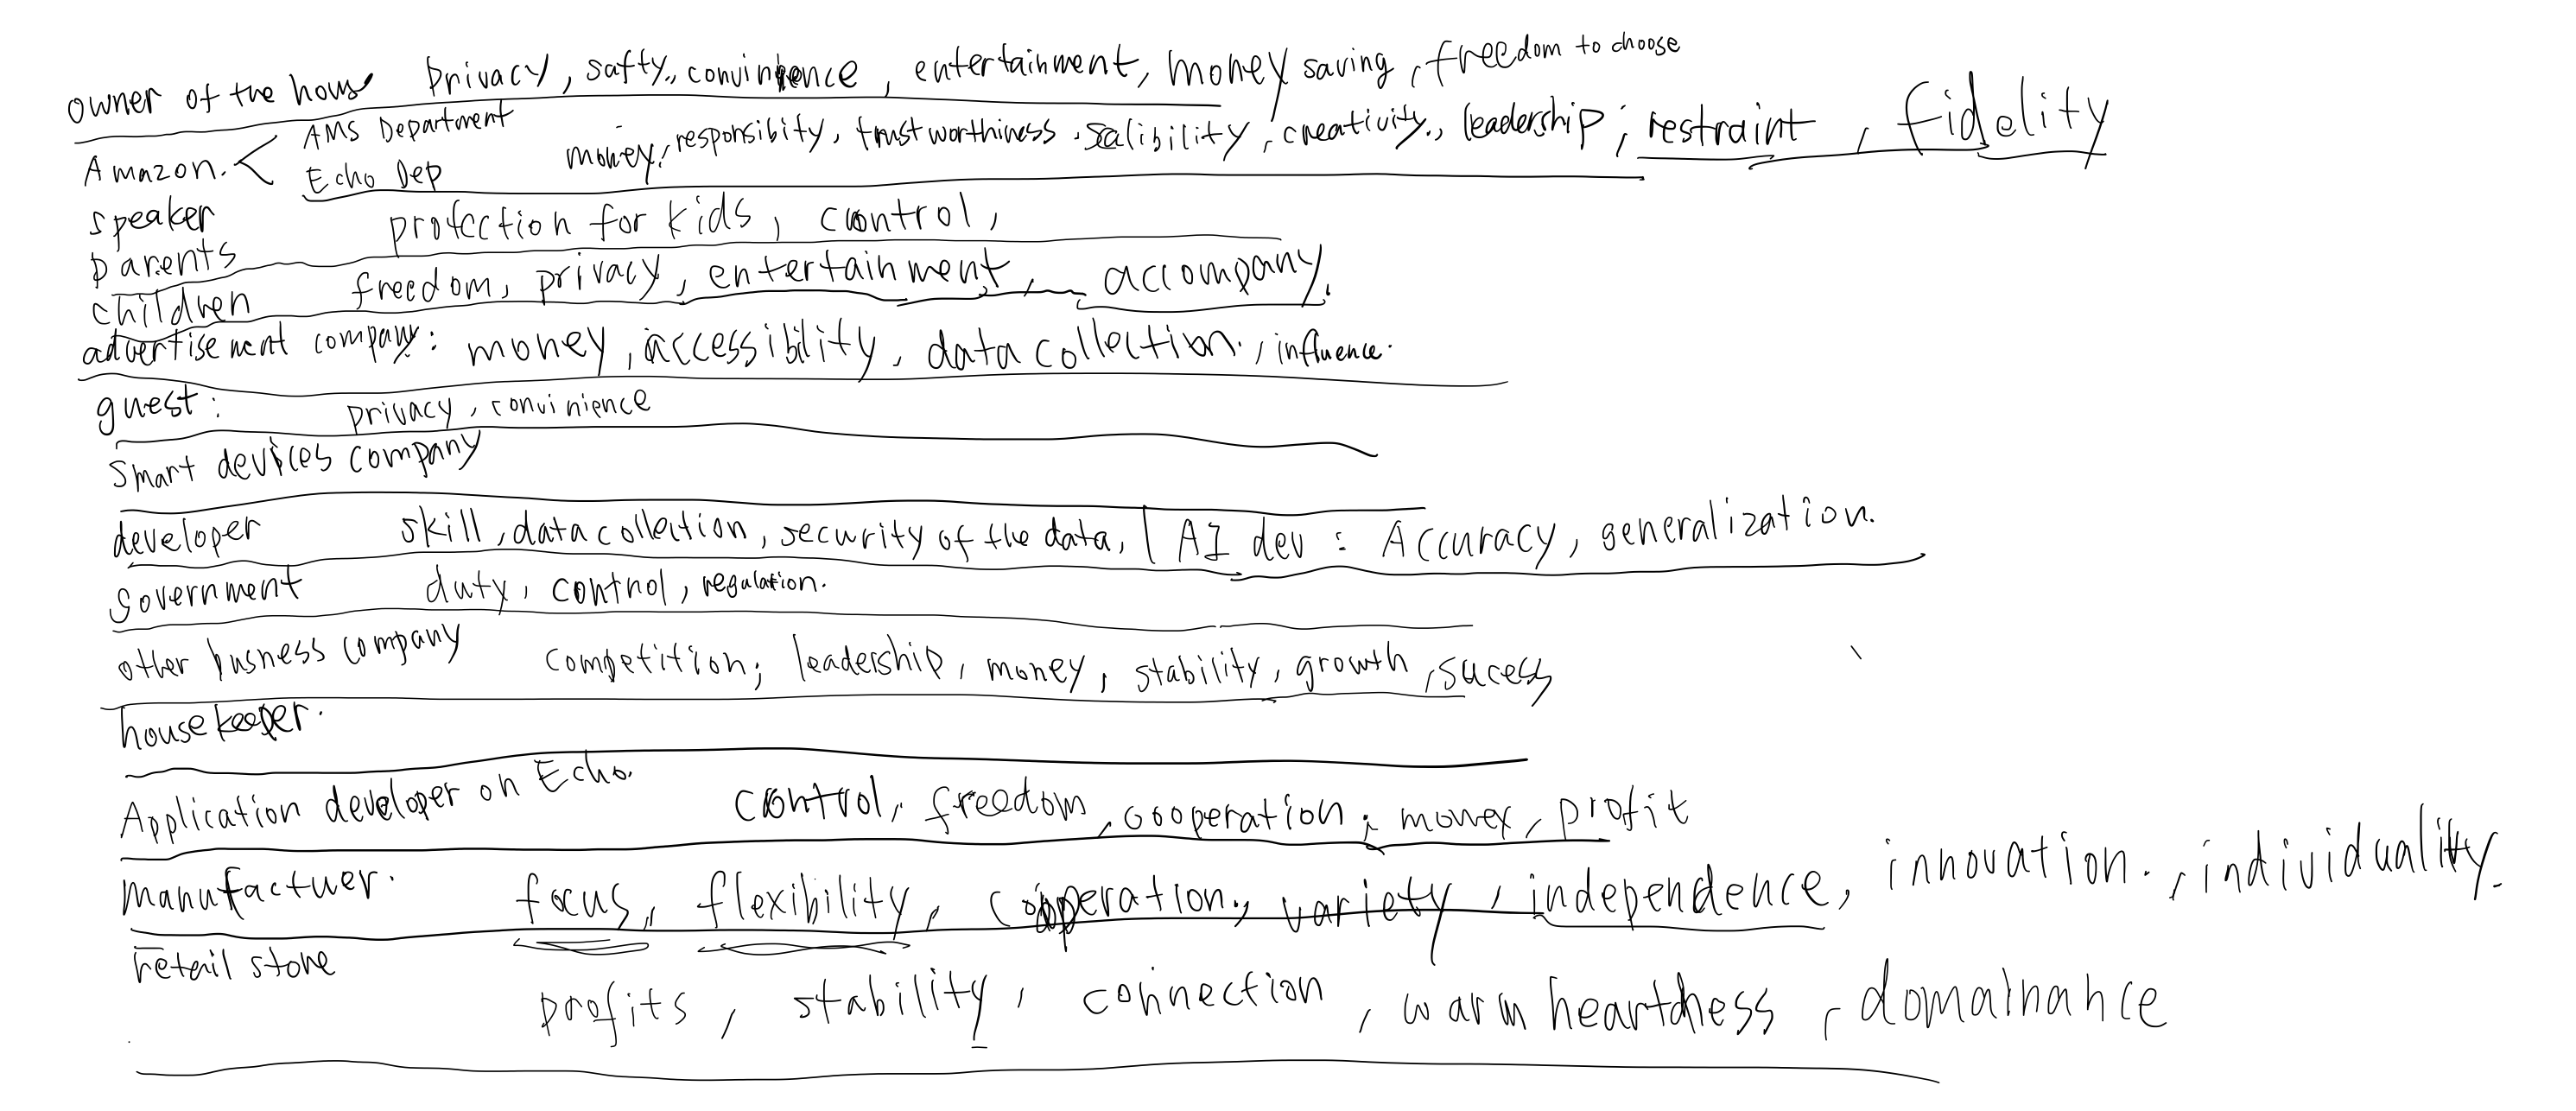
\includegraphics[scale=0.3]{values_2.png}

In the next step, we re-analysized values and draw the value map.

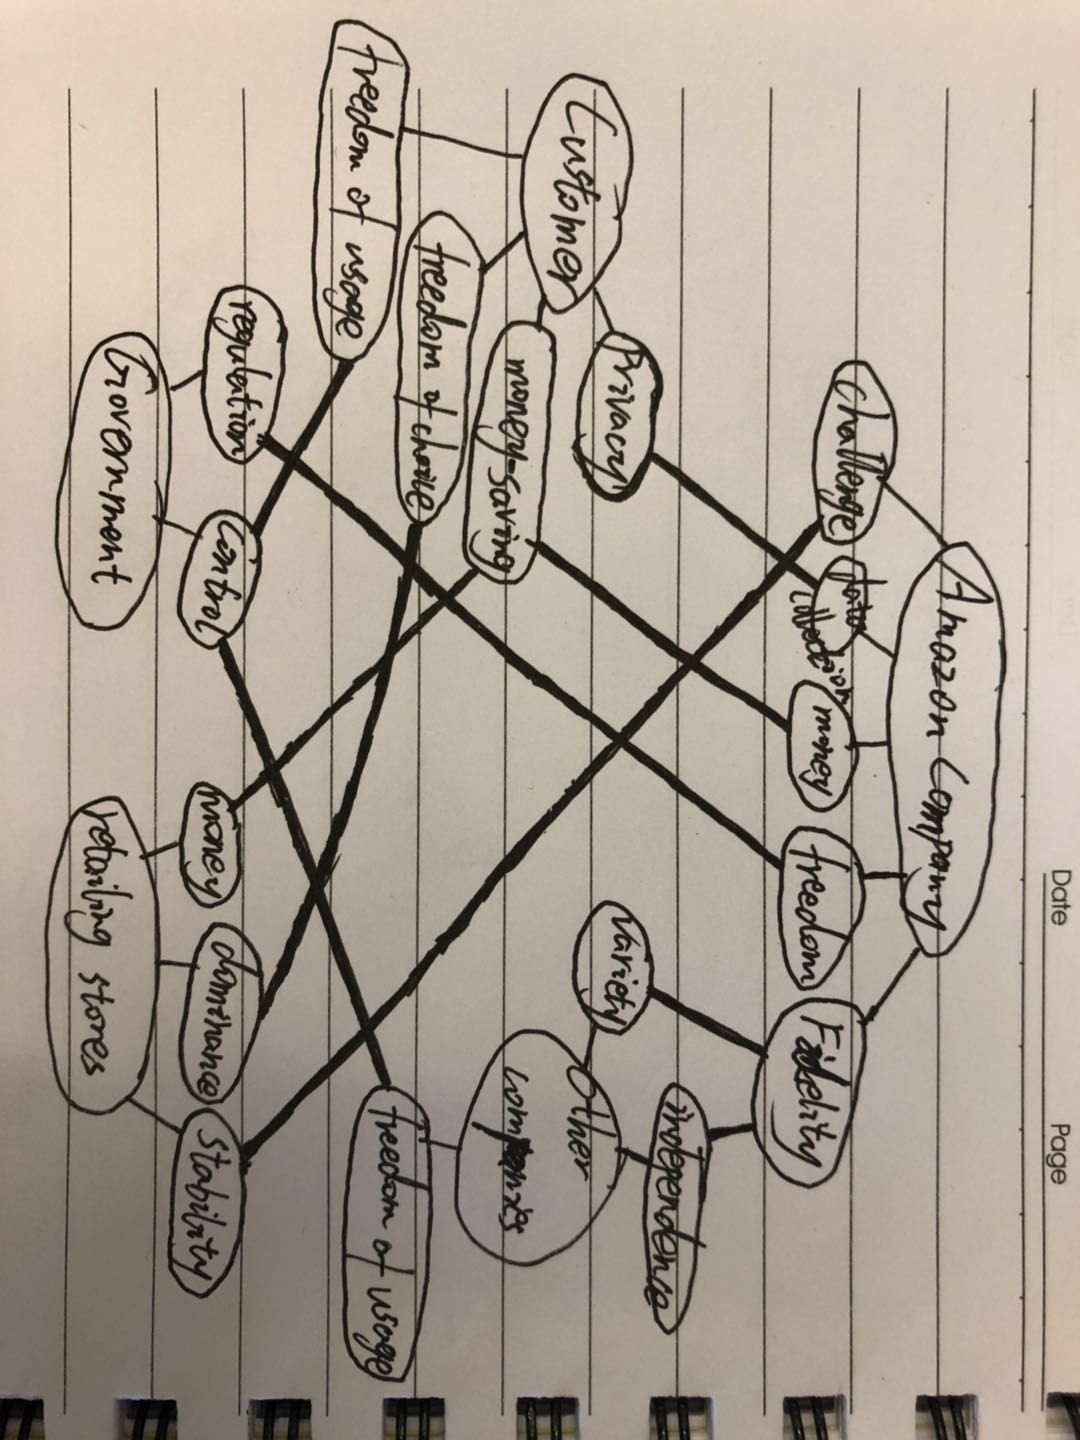
\includegraphics[scale=0.3,angle=90]{iter_1.jpeg}

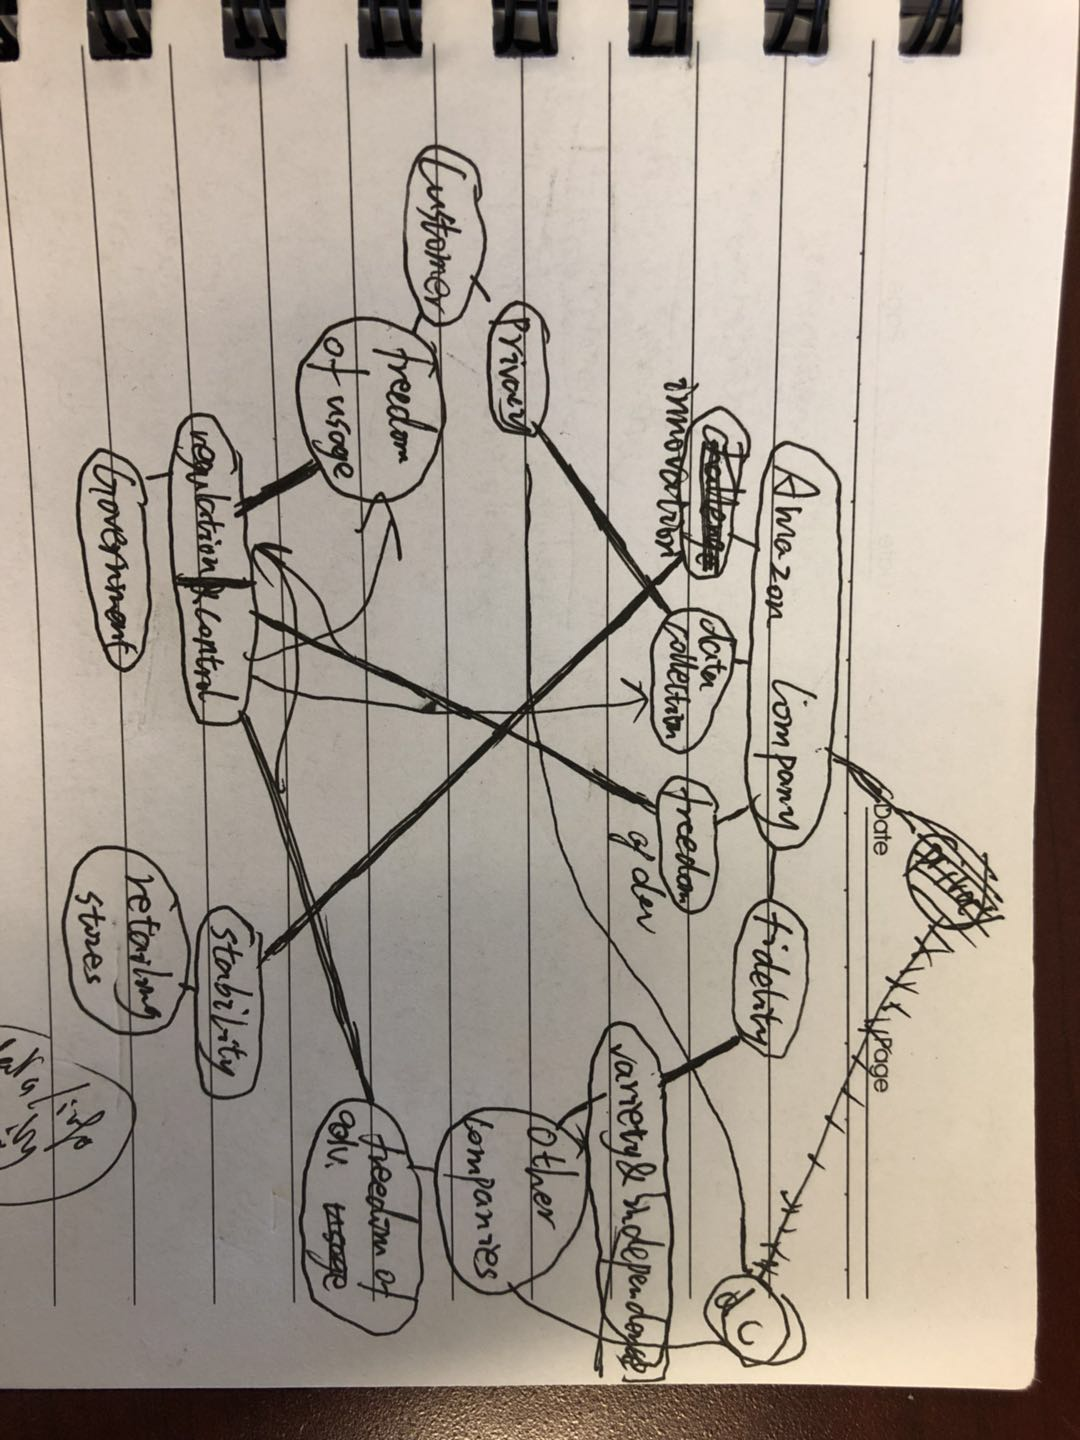
\includegraphics[scale=0.25,angle=90]{iter_2.jpeg}

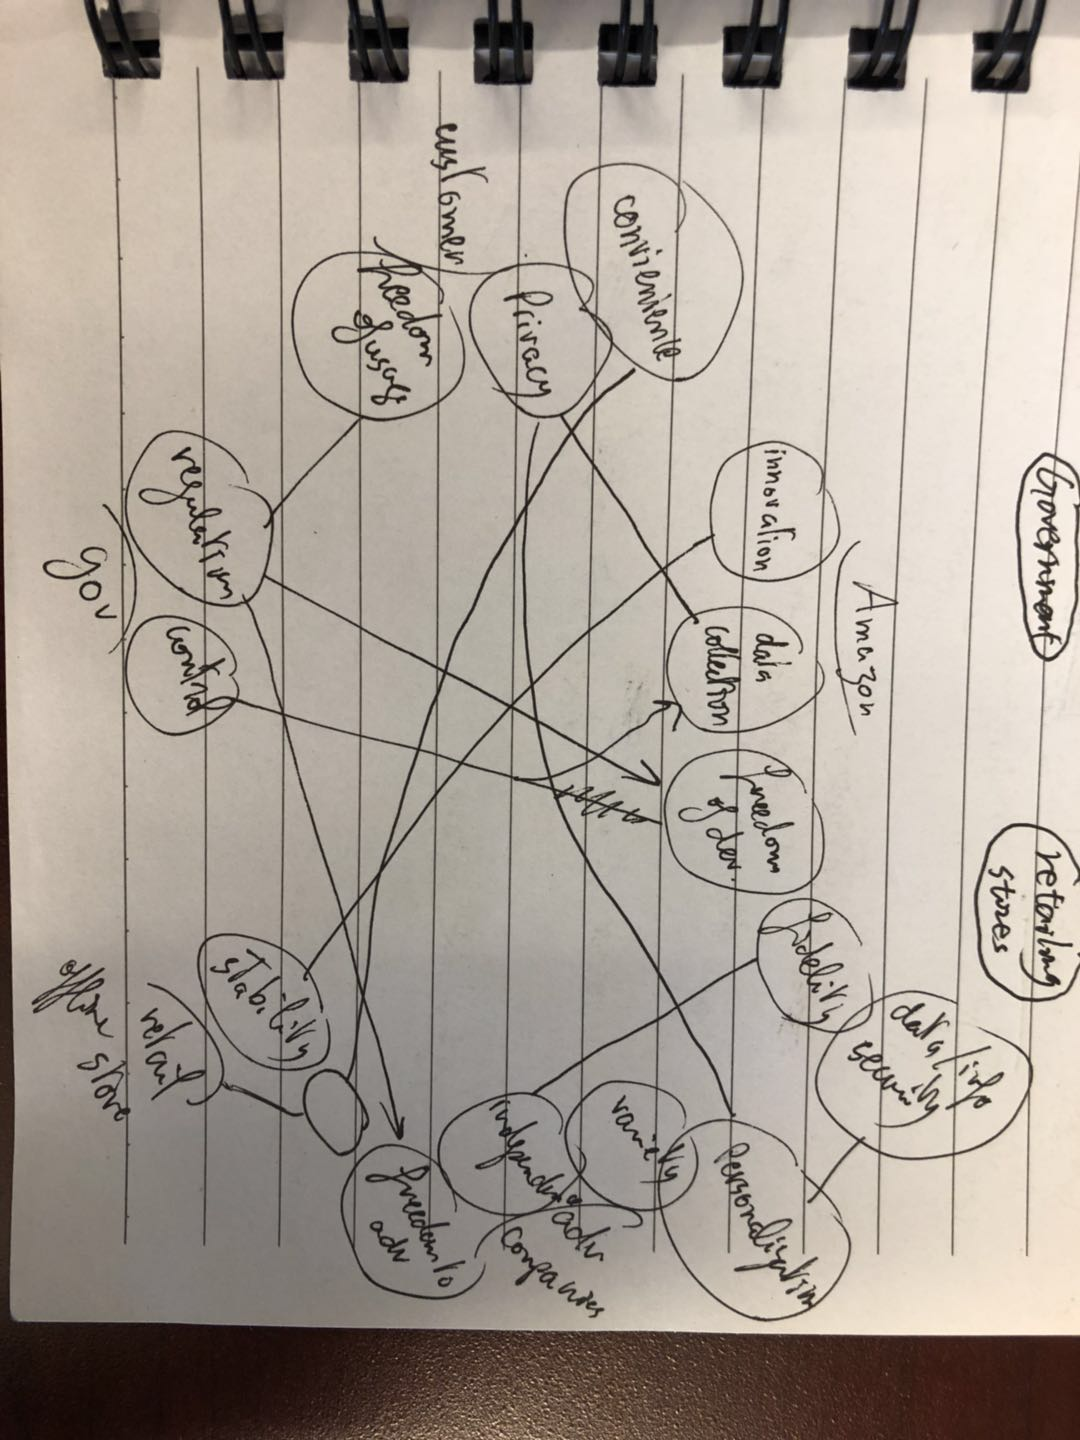
\includegraphics[scale=0.25,angle=90]{iter_3.jpeg}

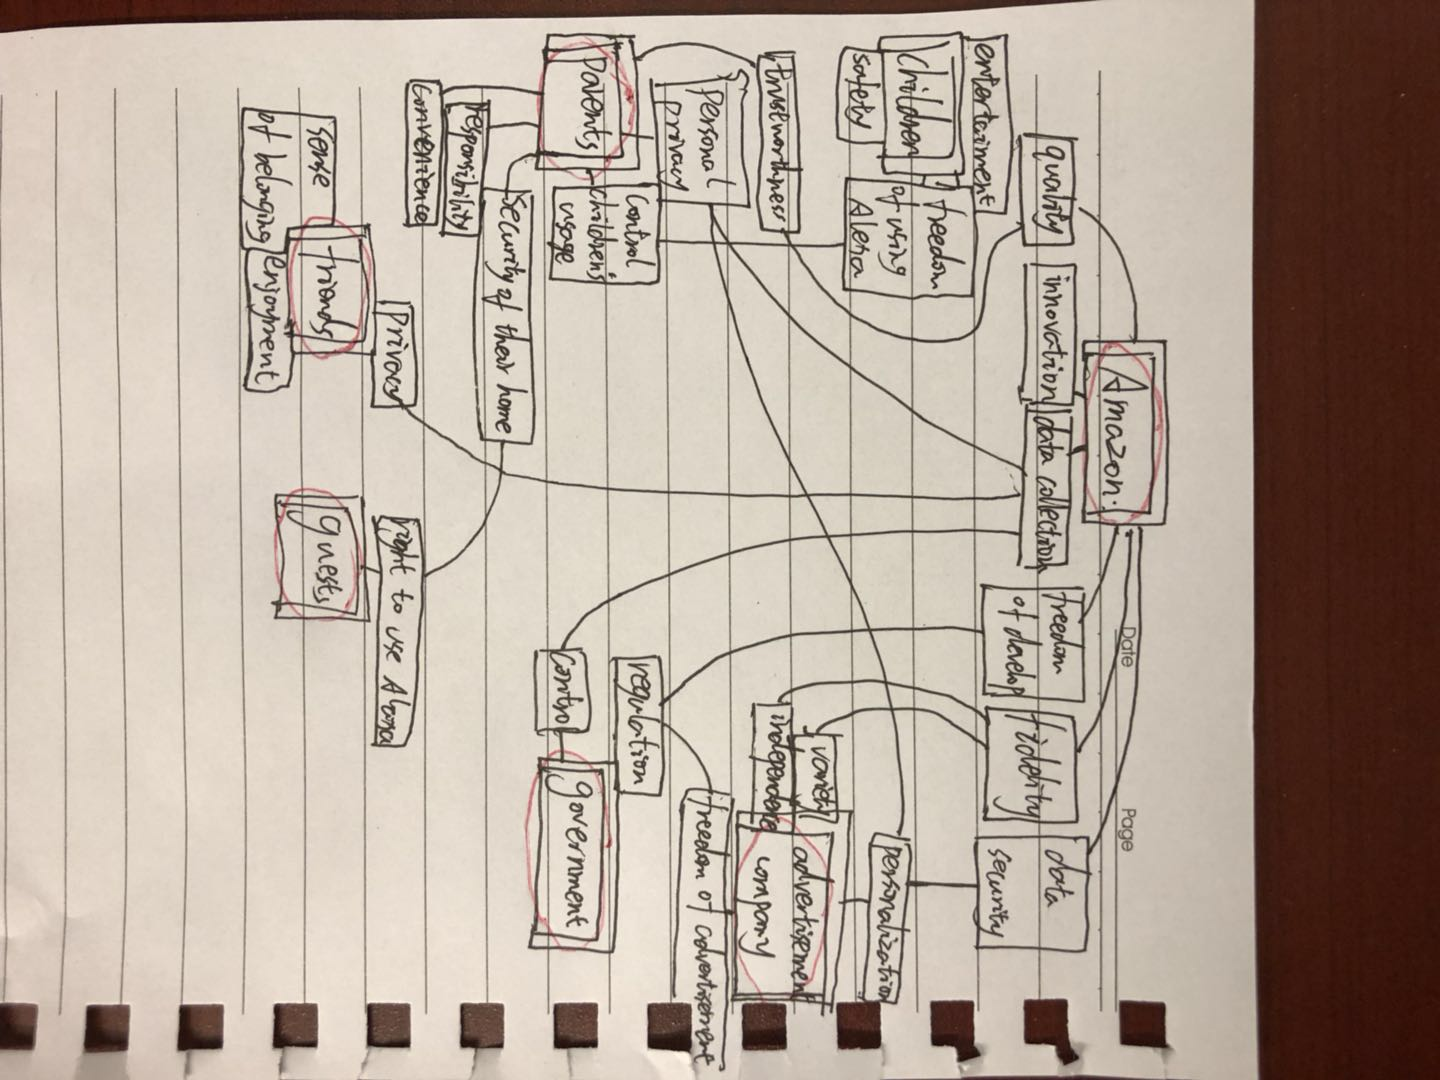
\includegraphics[scale=0.3,angle=90]{iter_4.jpeg}

We also consider the heatmap visulization method, each word represents the value, and value tensions are represented as combination of values. In addition, each color can show each stakeholder.

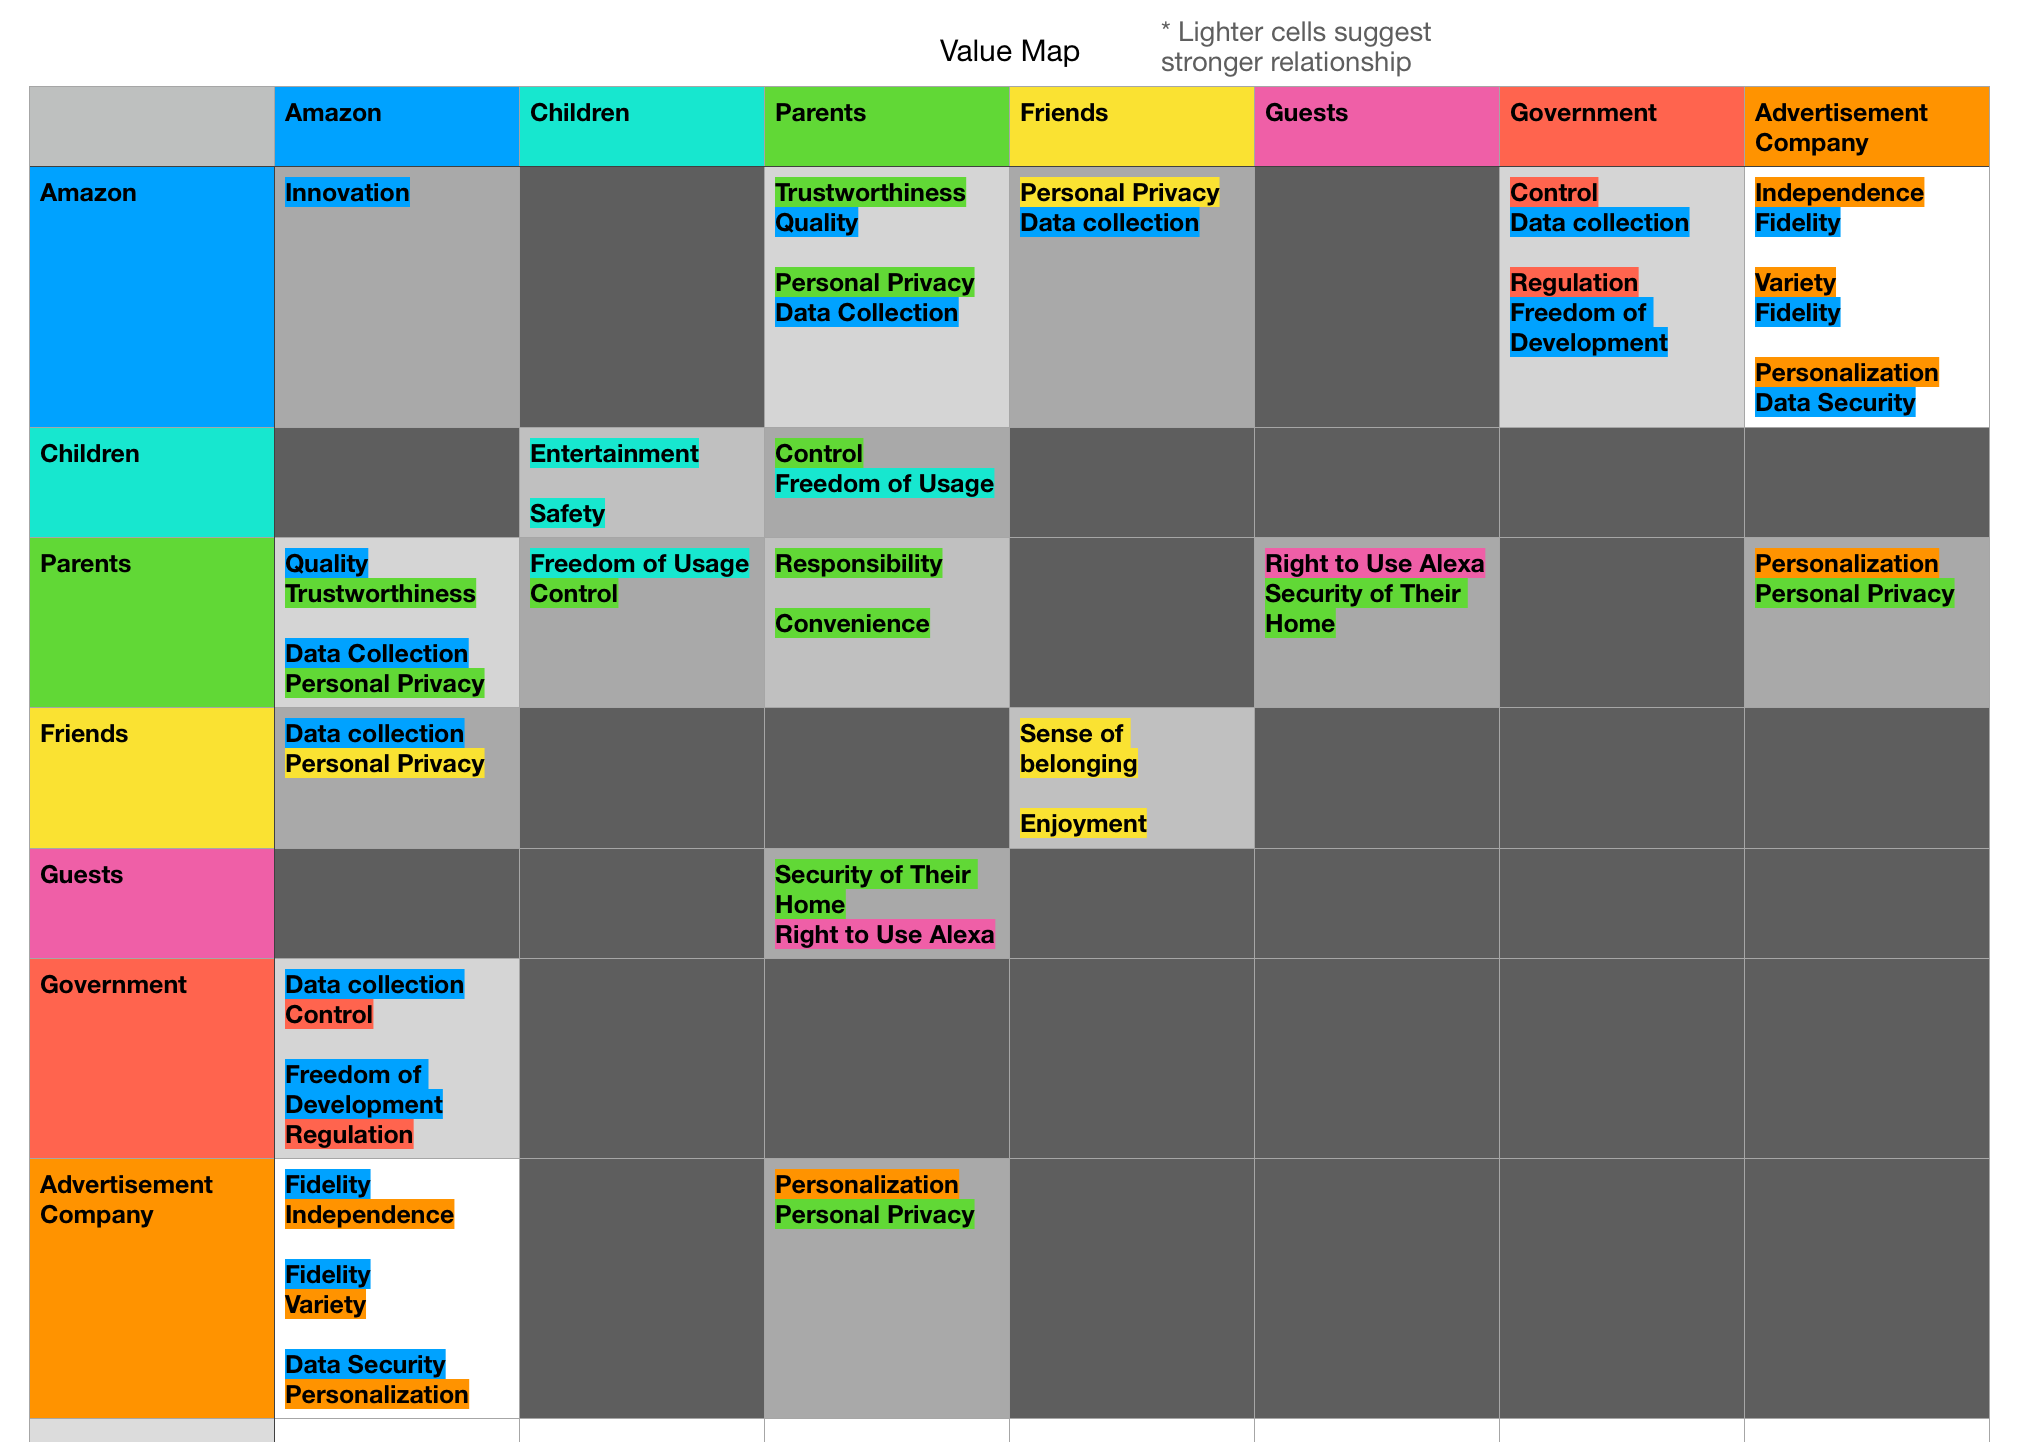
\includegraphics[scale=0.35]{heat_map_1.png}

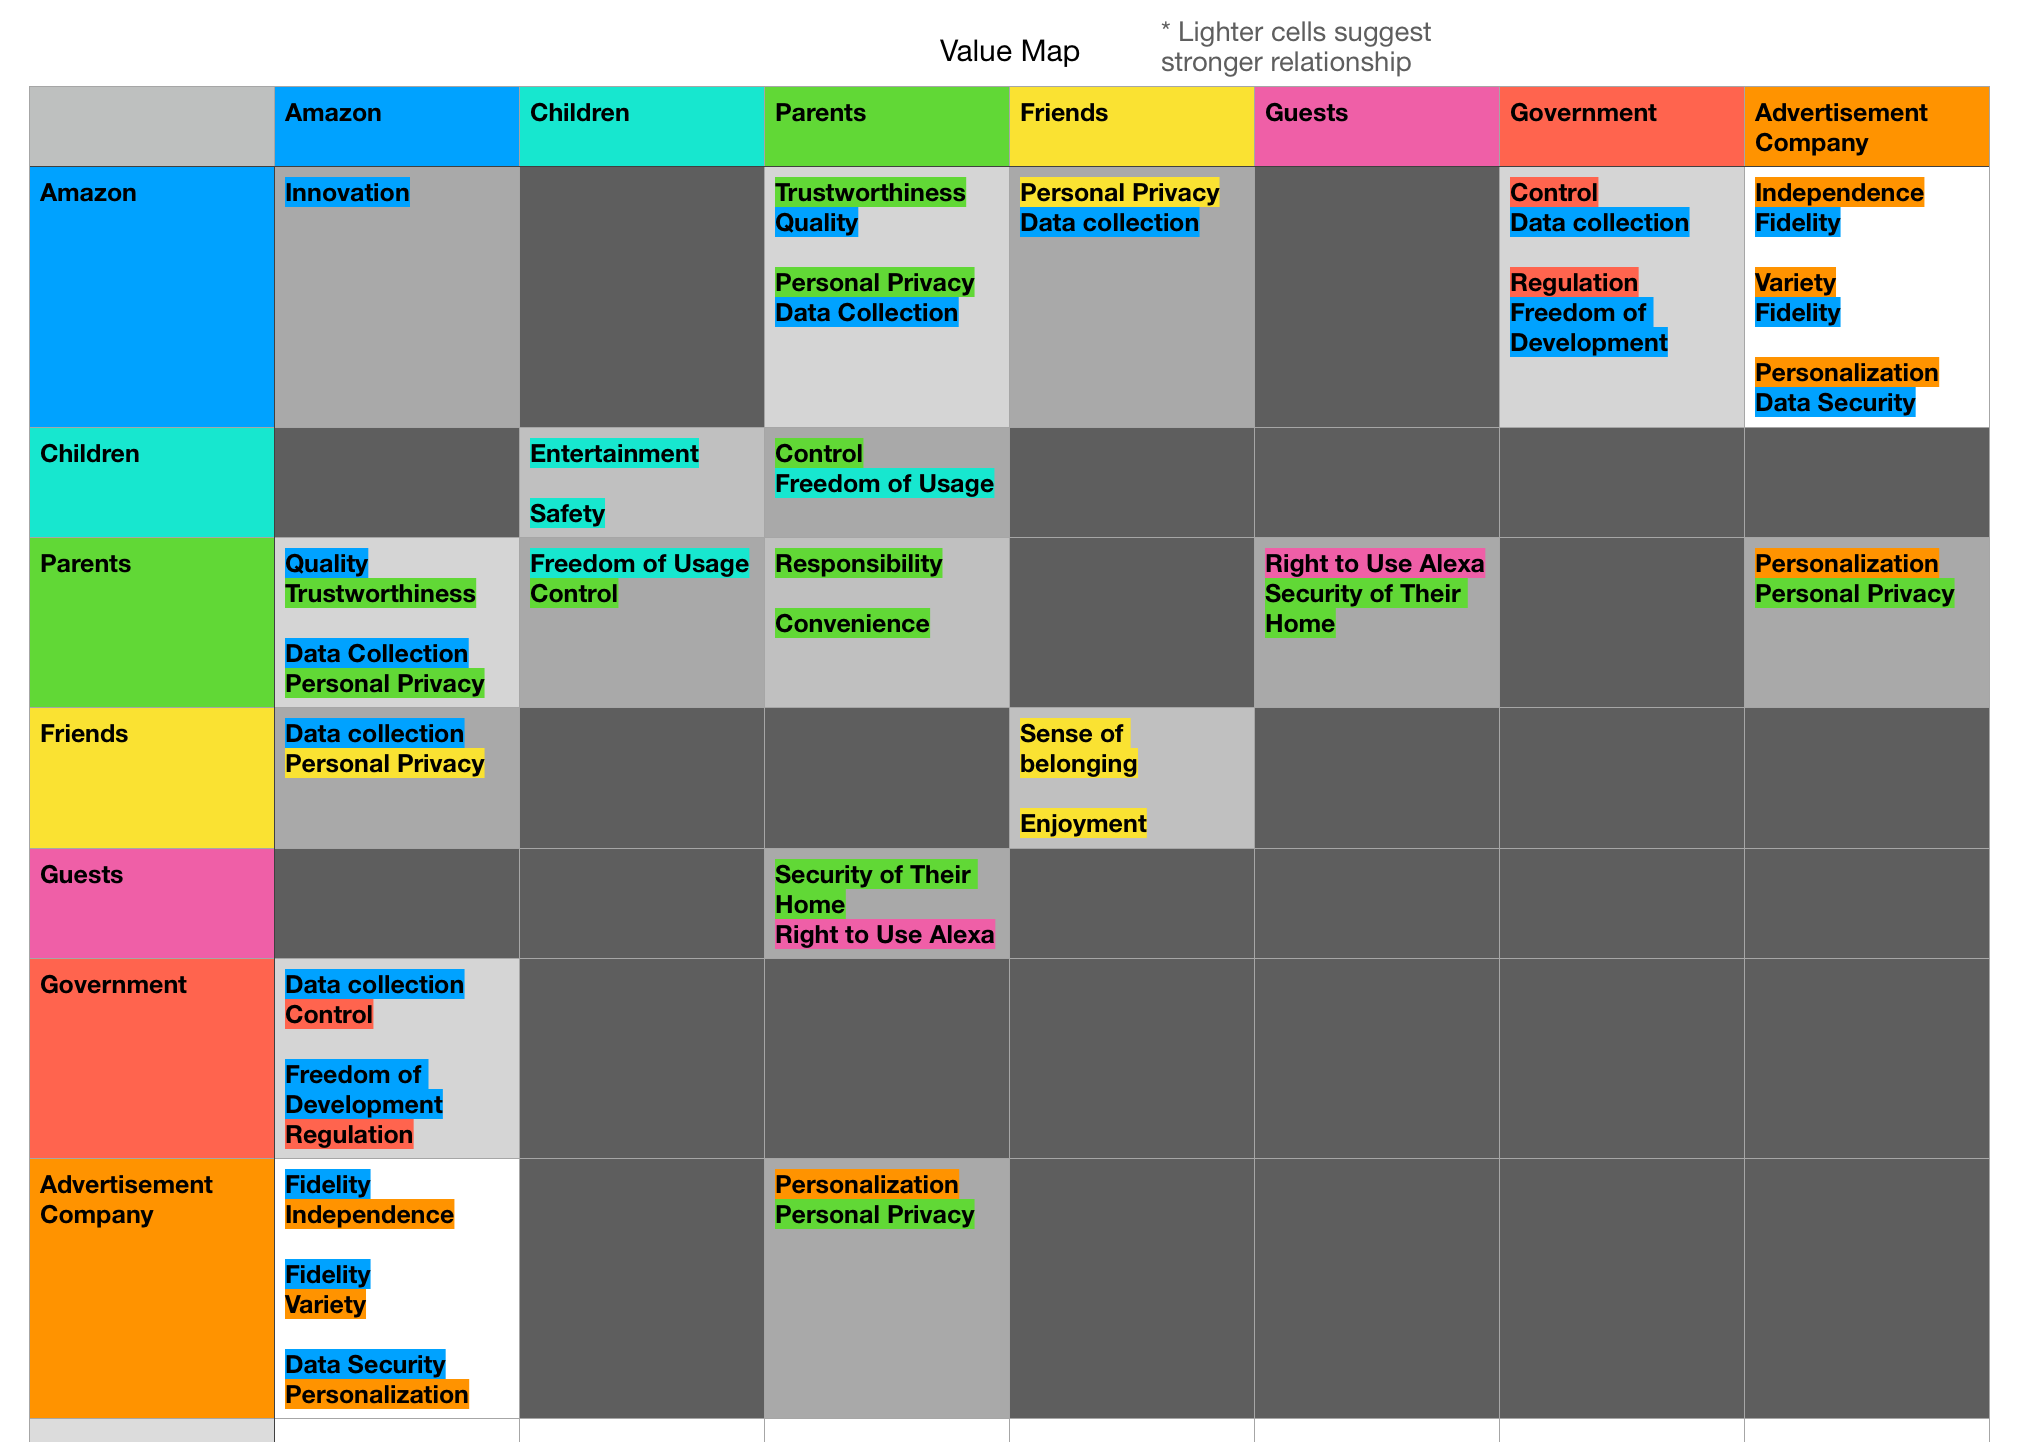
\includegraphics[scale=0.35]{heat_map_1.png}

Finally, we use google slides to build up our final value map, the below graph is a brief overview. More details please check link: \href{https://docs.google.com/presentation/d/1nQmXIbWmeZUNLPVEX4FJi_B35GRE-oLK9sPH9UOmlD0/edit?usp=sharing}{\url{https://docs.google.com/presentation/d/1nQmXIbWmeZUNLPVEX4FJi_B35GRE-oLK9sPH9UOmlD0/edit?usp=sharing}}. You can zoom in and out freely.

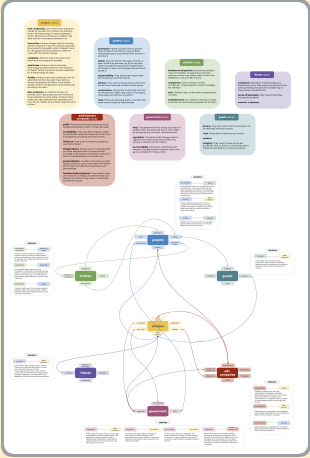
\includegraphics[scale=2]{final_value_map.png}

More details of draft graphs can be seen in .png and .jpeg source pictures.
\end{document}
